\documentclass[10pt]{IEEEtran}
\usepackage{graphicx}
\usepackage{float}
\usepackage{placeins}
\sloppy

\title{Skin Lesion Analysis Towards Melanoma Detection: Lesion Classification}

\author{Filipe Pires (85122) \& João Alegria (85048)}

\begin{document}
\maketitle

\begin{abstract}

In the past few decades cases of cancer have grown fast amongst humans. 
Even though many remain untreatable, an early detection of this kind of disease greatly increases the chances of treatment and survival.
The improvement of deep learning algorithms and intelligent image processing tools arrive as promising allies to cancer diagnosis processes, in particular cancer classification for skin and other visible body parts.

This report, written for a project on the course of Machine Learning, given by professor Pétia Georgieva at the University of Aveiro, aims to propose a form dealing with the classification of skin lesions into 3 unique diagnoses (melanoma, nevus, and seborrheic keratosis) based on deep neural networks working together. 
The purpose of the system developed was based on the ISIC Challenge of 2017 and uses the skin lesions datasets available online.

The validation score for the Melanoma Classifier was 0.80 and for the Seborrheic Keratosis Classifier was 0.75.
The system developed achieved a lower average accuracy score due to the combination process of the two classifiers.

\end{abstract}

\begin{IEEEkeywords}
Skin Lesion, Cancer Classification, Deep Learning, Convolutional Neural Network
\end{IEEEkeywords}

\section{\textbf{Introduction}} %%%%%%%%%%%%%%%%%%%%%%

The main goal of the challenge hosted by the International Skin Imaging Collaboration in 2017 was to encourage participants to develop image analysis tools to enable the automated diagnosis of melanoma from dermoscopic images. 

The image analysis of skin lesions was composed of 3 parts: lesion segmentation, detection and localization of visual dermoscopic features/patterns and disease classification. 
The datasets provided consisted of over 2000 images for training, 150 for validation and 600 for blind held-out testing.
In adition, the ISIC Archive (an international effort to improve melanoma diagnosis) contained the largest publicly available collection of quality controlled dermoscopic images of skin lesions available for any participant.

Our system focuses on the third part of the challenge, the skin disease classification, and follows the instructions and conditions of the challenge. 
Two independent binary image classifiers are used to diagnose each example: one for the classification of melanoma and non-melanoma cases and another for the classification of (seborrheic) keratosis and non-keratosis. 
The system integrates the decision of each classifier into one final answer (output): the prediction of the class to which an example belongs to of the 3 possible.

Our goal was to implement two Deep Neural Networks capable of correctly classifying the examples with an error as low as possible, focusing on studying the effects of several parameters and architecture characteristics of the model on its predictions.

\newpage{}
\section{\textbf{State of the Art Review}} %%%%%%%%%%%%%%%%%%%%%%

In this chapter we will discuss the 2 best solutions found for the skin lesion classification problem during the challenge and the strategies used by each. 
The technology and algorithms currently being used for tasks similar to this will also be described here.
But before proceding, it is important to give some important definitions mentioned in this report and a background about the matter at hands.

\subsection{Machine Learning Models \& Statistical Algorithms}

As the most common model for machine learning through image analysis is Deep Neural Networks, the basic definitions of this type of model and subtypes are given below.

\begin{itemize}
\item \textbf{Artificial Neural Network (ANN)} - also known as a neural network, it is a computational model based on the structure and functions of biological neural networks. Information that flows through the network affects the structure of the ANN because it changes - or learns, in a sense - based on that input and output. ANNs are considered nonlinear statistical data modeling tools where the complex relationships between inputs and outputs are modeled or patterns are found.
\item \textbf{Deep Neural Network (DNN)} - it is an ANN with a certain level of complexity, a neural network with more than two layers. DNNs use sophisticated mathematical modeling to process data in complex ways.
\item \textbf{Convolutional Neural Network (CNN)} -  also known as a ConvNet, it is a specific type of DNN that uses perceptrons for supervised learning to analyze data. CNNs apply to image processing, natural language processing and other kinds of cognitive tasks.
\end{itemize}

Other models are mentioned in this report, their definition is present here.

\begin{itemize}
\item \textbf{Decision Tree (DT)} - it builds classification or regression models in the form of a tree structure. It breaks down a dataset into smaller and smaller subsets while at the same time an associated decision tree is incrementally developed. The final result is a tree with decision nodes and leaf nodes. Decision trees can handle both categorical and numerical data. 
\item \textbf{Support Vector Machine (SVM)} - it is a machine learning model that maximizes the margin around the decision surface (or hyperplane) that separates examples represented in space. The decision function is fully specified by a (usually very small) subset of training samples, the support vectors. Support vectors are the data points that lie closest to the hyperplane.
\end{itemize}

A few algorithms are also mentioned. We offer a basic understanding of them in order for the reader to follow more easily.

\begin{itemize}
\item \textbf{Perceptron} - it is a machine learning algorithm that helps provide classified outcomes for computing. It takes a set of inputs and returns a set of outputs. These are often presented visually in charts for users.
\item \textbf{Random Forest (RF)} - it is a supervised learning algorithm where a creation of a forest somehow made random takes place. The "forest" it builds is an ensemble of DTs, most of the time trained with the “bagging” method. The general idea of the bagging method is that a combination of learning models increases the overall result.
\item \textbf{Softmax} - it is a machine learning algorithm that assigns decimal probabilities to each class in a multi-class problem. Those decimal probabilities must add up to 1.0. This additional constraint helps training converge more quickly than it otherwise would. Softmax is an extension of the idea of Logistic Regression into a multiclass world.
\item \textbf{Principal Component Analysis (PCA)} - it is a technique used for identification of a smaller number of uncorrelated variables known as principal components from a larger set of data. The technique is widely used to emphasize variation and capture strong patterns in a data set. It helps make data easier to explore and visualize.
\end{itemize}

Aditional helpful definitions:

\begin{itemize}
\item \textbf{Hyperparameter} - model hyperparameters are the properties that govern the entire training process. The variables usually configure before training a model are: Learning Rate (or Lambda), number of Epochs, Hidden Layers, Hidden Units, Activations Functions. 
\item \textbf{Evaluation Metrics} - they are the basis of the evaluation of a machine learning model. Since each machine learning model is trying to solve a problem with a different objective using a different dataset, it is important to understand the context before choosing a metric of evaluation. As the problems referred in this report are all of classifications, the only metrics mentioned will be the ones of this context. The most common are: accuracy, precision-recall (specificity-sensitivity), f1 score, log-loss, etc.
\end{itemize}

\begin{figure}[H]
\centering
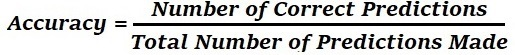
\includegraphics[width=6cm]{AccuracyMetric.jpg}
\caption{Used evaluation metric formula.}
\end{figure}
\newpage{}

\subsection{Skin Legions}

In order to appropriately follow the study, one must understand the fundamental concepts related to skin lesions and diseases.
A summarized definition of the 3 classes of diseases mentioned in this study is present below:

\begin{itemize}
\item \textbf{Melanoma} - a type of cancer that develops from the pigment-containing cells and is primarily caused by excessive exposure to ultraviolet light. It is the deadliest form of skin cancer, responsible for over 9,000 deaths each year. 
\item \textbf{Nevus} - a type of skin mole typically harmless and very common. In some cases it may become cancerous and should be removed.
\item \textbf{Seborrheic Keratosis} - a type of skin growth completly harmless. It is sometimes difficult to distinguish from a melanoma case.
\end{itemize}

The typical form of analysing skin and diagnosing diseases is based on the experience of a dermatologist doctor. 
He or she may collect samples for a deeper analysis but the process requires the full attention of a specialized person.

The possibility of the development of a tool that could help a professional better diagnose cases such as the melanoma cancer and decrease the waiting time of the process is much desired.
In the past decade, with the growth of the field of machine learning and the improvement of the processing capacity of computers and image processing algorithms, some solutions have started to emerge as usefull tools in areas such as medicine.
Today, the studies conducted are dedicated to the improvement of computer vision systems and deep learning algorithms in order to increase the accuracy of such tools and make them more reliable.
The ISIC Challenge is a great example of initiatives aiming towards this goal and benefiting the society in general.

\subsection{Best Solutions of the ISIC Challenge of 2017}

This subsection will be dedicated to the analysis of the strategies used by 2 of the winning teams of the ISIC Challenge in the year of 2017. 
They will serve as useful examples of the current state of the art in the field of deep learning and cancer classification.
\newline{}

\textbf{ResNet Ensemble with Normalized Image}

Casio and Shinshu University joint team, composed by K. Matsunaga, A. Hamada, A. Minagawa and H. Koga, proposes a method that focuses intensily on a preprocessing phase in order to improve the prediction accuracy.
The team decided to run a normalization of the luminance and color balance of input images exploiting color constancy before feeding the data to their classification system. 

Taking in consideration that the cases os keratosis and melanoma were few amongst the entire dataset, they decided to geometrically transform the images in order to increase the number of examples good for the learning process.
The age and sex information available about some examples was also used in the learning process, adopting a straightforward thresholding only for one classifier.
Aditional training data was gathered from the external subset of the ISIC Archive. 

The transformed images are input in parallel to an ensemble of Convolutional Neural Networks (CNNs) and a prediction value in [0.0,1.0] is output.
The networks have an architecture of 50-layer ResNet (Deep Residual Learning).

The evaluation results were very positive, with an mean accuracy score of 0.911 for the model predictions. 
Though not mentioned by the authors, we believe that the image normalization and transformations had a great impact on the performance of the system, reducing the errors related to images taken under different setups and increasing the number of good learning examples.
This work is a good example of the importance of preprocessing data when needed.

\begin{figure}[H]
\centering
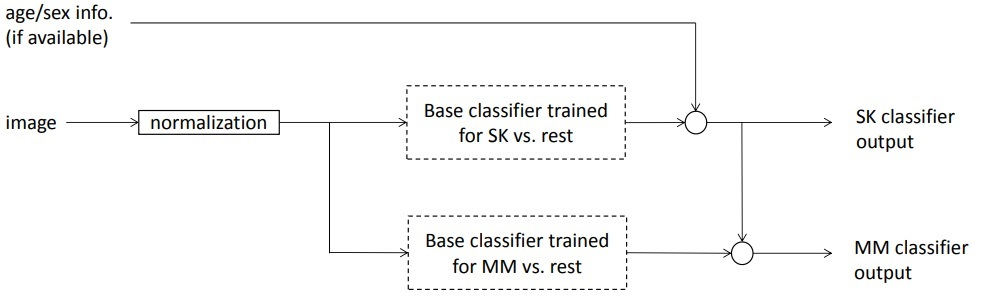
\includegraphics[width=9cm]{ISIC_1stPlace_ClassificationSystem.jpg}
\caption{Classification System proposed by the Casio and Shinshu University joint team.}
\end{figure}

\textbf{gpm-LSSSD}

Iván González-Díaz, of the Multimedia Processing group of the University Carlos III of Madrid, proposes a more complex solution yet with an almost equal accuracy score of 0.910.
His approach incorporates the expert knowledge of dermatologists into the well known framework of CNNs. 
The system contains several networks providing lesion area identification, lesion segmentation into structural patterns and final diagnosis of clinical cases.

The high performance of this model is largely benefited by the 2 initial strategies. 
In a way, the lesion segmentation network serves as a preprocessing step along with the image transformations that this solution shares with the ResNet one. 
The complex architecture of the diagnosis network (the final network of the model) takes advantage of well known algorithms such as Softmax to increase the quality of the system's predictions.

\begin{figure}[H]
\centering
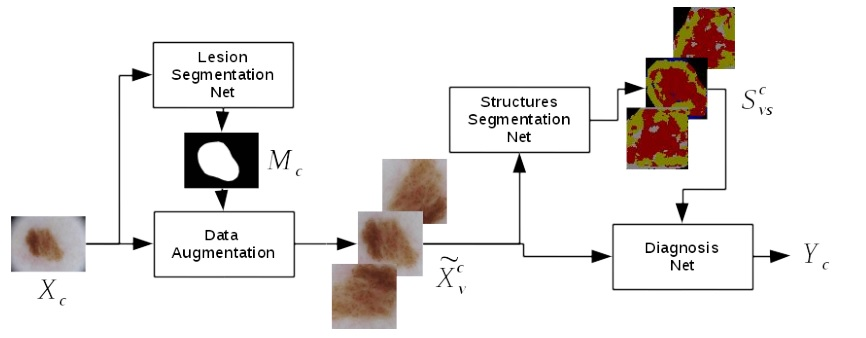
\includegraphics[width=9cm]{ISIC_2ndPlace_ClassificationSystem.jpg}
\caption{Main processing pipeline of the Classification System proposed by the Multimedia Processing member.}
\end{figure}
\newpage{}

\subsection{Disease Learning Through Image Processing}

Most of the machine learning models being developed for health-related situations are based on some kind of image processing, whether it is conventional 2D images or 3D visualizations.
In this subsection, some of the most common strategies of models using deep neural network that learn through images are covered.

\textbf{Convolutional Neural Network Algorithm with Parameterized Activation Function for Melanoma Classification}

This paper published by Abdulaziz Namozov and Young Im Cho, from Gachon University, Korea has the main objective of proving that the activation layers in Deep Neural Networks have a very important role in the model's performance.
It shares with the previous papers the characteristic of being originated from the participation of the two investigators in the ISIC Challenge (this time, in the 2018 competition).

From a dataset supplied by the ISIC Archive about Skin Lesion Analysis towards Melanoma Detection (2018), the authors proceeded to ilustrate the hypothesis they had by testing and training multiple CNN with different activation layers, while maintaining the remaining hyperparamenters. The model's architecture consisted of 9 layers, 4 convolutional and 3 fully connected in the end for classification, making the activation layers the only thing responsable for any changes in the outcome.

The conlusions reached by the article are to be considered in future studies because, as defended by the authors, the adaptive piecewise linear activation (APL), a specific activation mode, revealed to be better in their case against classical activations like rectified linear unit activation (ReLU) or tangent activation obtaining (with data augmentation) an accuracy of 95,86\%, 93,25\% and 91,76\% respectively.

\textbf{Ultrasound Text Classifier for Predicting Benign and Malignant Thyroid Nodules}

This publication of the International Conference on Green Informatics differs from the others in the sense that it describes a machine learning model that learns from ultrassound data instead of processed surface images (like skin pictures).
The team of developers from the Donghua University, China, tackled the classification problem of benign and malignant thyroid nodules with a structured analisys approach based on dependency syntax analysis.

The data collected from recording pacients speaking was fed to a deep neural network along with clinical information. 
To reduce the distortion caused by overlapping information,they used PCA to select and remove unnecessary features.
The learning rate was adaptive and the hyperparameters studied were the number of hidden layers and of hidden layer nodes. 

The team tested their dataset for the DNN and 3 other rival models (NN, RF, SVM). The DNN showed higher values for the precision, recall and f1 metrics and reaching an accuracy of 93\%.

\textbf{Automatic Detection of Cerebral Microbleeds From MR Images via 3D Convolutional Neural Networks}

Published in the IEEE Transactions on Medical Imaging, this study can be considerer as a pionner in the area where it applies, since the team of developers explores the concept of 3D CNNs, a technology not yet extensively explored.
The team from the Chinese University of Hong Kong and the Shenzhen University, China, were interested in automating the detection of Cerebral Microbleeds.
 For that, they relied in MRIs (Magnetic Ressonance Images), which basically consists in various layers of images, each one corresponding to a layer of the brain examined, giving this type of exam a 3D characteristic.

The authors mention that in previous investigations the methodology consisted in training a CNN with the exam images, considering each layer image as independent from the others. 
But they came up to the conclusion that such approach does not consider some important information and relations, because it completly removes the notion of the specific characteristic of 3D in this type of exams. 
For this reason, the chinese team decided to use a 3D CNN, taking in consideration the full dimension of the data. 
However, that approuch is very expensive, requiring a lot of resources such as computational capacity, memory space and execution time. 
To reduce this cost, the study proceded with a cascade framework, applying first a 3D FCN (Fully Convolutional Network, a network only composed by convolutional layers) to rapidly retrieve potencial candidates and then feeding the output candidates to a 3D CNN to single out the true CMB(Cerebral Microbleeds) from the hard mimics.

With a considerably large dataset with 320 volumetric MR scans and performing extensive experiments to validate the proposed method, the article authors achieved a high recall (sensitivity) of 93.16\% with an average number of 2.74 false positives per subject, outperforming previous methods using low-level descriptors or 2D CNNs by a significant margin. 
The proposed method, in principle, can be adapted to other biomarker detection tasks from volumetric medical data. 
This article turns out to be very important not only for the technologies used and explored but also the fact that it can be adapted to many other contexts. 

\begin{figure}[H]
\centering
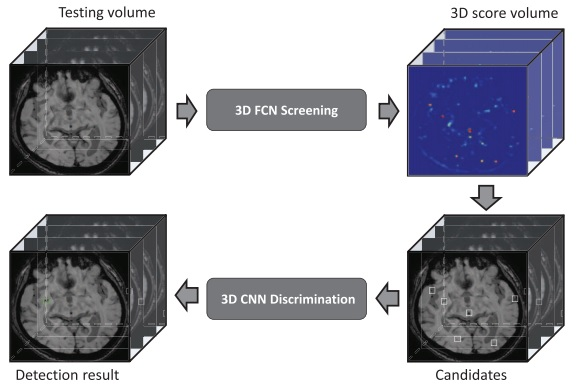
\includegraphics[width=9cm]{CMBDetection_CascadeFramework.jpg}
\caption{Cascaded Framework for CMB Detection proposed by the article authors.}
\end{figure}
\newpage{}

\section{\textbf{Data Description \& Preprocessing}} %%%%%%%%%%%%%%%%%%%%%%

\subsection{Statistical Analysis \& Visualization}

Lesion classification data made available by the ISIC coordination team includes of a large set of dermoscopic lesion images in JPEG format and two CSV files, one with some clinical metadata for each image. 
The data consists of the original image of a skin lesion, paired with a gold standard (definitive) diagnosis, referred to as "Ground Truth" (and present in the second CSV file).

2000 images are provided as training data, including 374 melanoma, 254 seborrheic keratosis, and the remainder as benign nevi (1372).
Figure \ref{fig:datadistribution1} shows the distribution of each diagnosed disease.
The CSV file containing the metadata for each image is composed of 3 columns: the image identifier, the age of the lesion patient rounded to 5 year intervals (or "unknown") and the sex of the lesion patient (or "unknown").

The Training Ground Truth file is a single CSV file, containing 3 columns: a word with the image identifier and the remaining columns with an integer between 1 and 0.
These binary-valued columns represent the two binary classification tasks (melanoma vs. nevus and seborrheic keratosis and seborrheic keratosis vs. melanoma and nevus).

According to the ISIC Challenge coordination team, malignancy diagnosis data were obtained from expert consensus and pathology report information.

After manually analysing the dataset, some observations were made.
It was very clear that the sources where the images were taken from and the lighting and environment context where each picture was taken varied throughout the entire set.
Some examples of the discrepancy between images are present in figure \ref{fig:skinlesions}.

Along with all the dermoscopic lesion images, a PNG file was also made available for each image. 
These files, referred to as "superpixels", seem to contain information about each image. 
However, since no referrence to them is given in the ISIC Challenge and the images alone are not sufficient to understand their meaning, these were not considered for this report's study.
\newpage{}

\subsection{Data Preprocessing}
\label{dp}

After analysing all available data and the disposable computational capacity for this study, some decisions were made regarding the 2000 images.

The first step was to rescale all images to a resolution equal for the entire set. 
For this, a search for the most frequent resolution took place in order to distort the least amount of images possible. 
After that, all other images with a different resolution were resized to fit the chosen one.

During the first tests over an initial DNN for the first classifier, some problems occurred due to the high demand of computational capacity made by the training process.
As the images were too large, the machine were the system ran was not able to process all information in an acceptable amount of time.
As a consequence, all images suffered a second resize operations in order to reduce the space used by each.
Here, two different approaches were tested: one would resize keeping the most common heigth-width ratio, the other would resize all images to a ratio of 1:1.
As no difference in performance was detected between the two approaches, the second one was chosen for practical reasons.
At the end of this second step, the resolution of all training images was 200x200 pixels. 
However, as it is mentioned in chapter \ref{pae}, this size was varied and tested as a hyperparameter for the machine learning model.

The third step was introduced after reading the report of the Casio and Shinshu University joint team for the ISIC Challenge of 2017.
The team mentions that a color correction was applied to all images in order to increase the overall similarity and decrease the error associated with the varying context where each picture of a skin lesion was taken.
Taking this possible source of error in consideration, we decided to run a normalization process exploiting color constancy called Gray World. 
This method is among the simplest illuminant estimation methods. The main premise behind it is that in a normal well color balanced photo, the average of all the colors is a neutral gray. Therefore, we can estimate the illuminant color cast by looking at the average color and comparing it to gray.

The fourth and final step took in consideration only the known cases of melanoma and of seborrheic keratosis (which were in total 628).
The idea here exploits the fact that the DNNs search for patterns in the images and that the patterns found in each lesion could appear in the exact same position but rotated or inversed.
In theory, if the same images were fed to a DNN several times rotated in different angles, the classifier would gain a better understanding of the patterns present in the malignant lesions.
We tested out 3 rotations to the right for each original image: 90º, 180º and 270º. 
This resulted in a total of 1496 images of melanoma and 1016 images of seborrheic keratosis.
Figure \ref{fig:datadistribution2} shows the distribution of each diagnosed disease after adding the new images to the training dataset.
Even though this process could be done to all 2000 images, since the time for completing this study was very limited, we decided to apply it only to the mentioned cases because it would save time while feeding the DNNs more information of positive cases.
\newpage{}

\begin{figure}[H]
\centering
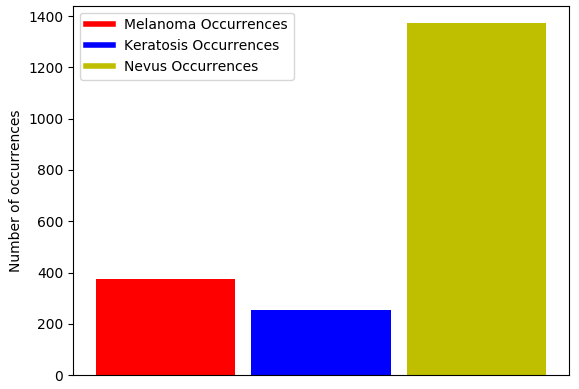
\includegraphics[width=8cm]{ISIC_DataClassificationDistribution.jpg}
\caption{Distribution of the 2000 images amongst the considered classes.}
\label{fig:datadistribution1}
\end{figure}

\begin{figure}[H]
\centering
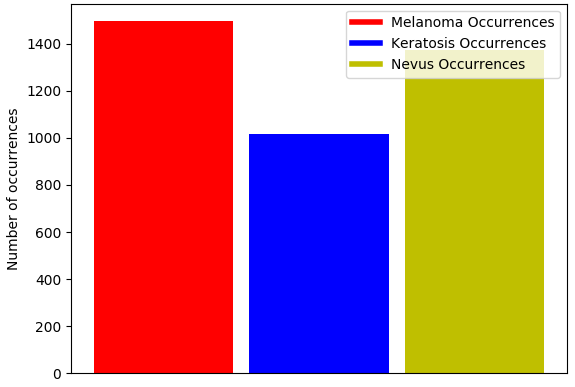
\includegraphics[width=8cm]{ISIC_DataClassificationDistribution_Rotations.jpg}
\caption{Distribution of the entire dataset (3884 images) amongst the considered classes after preprocessing.}
\label{fig:datadistribution2}
\end{figure}

\begin{figure}[H]
\centering
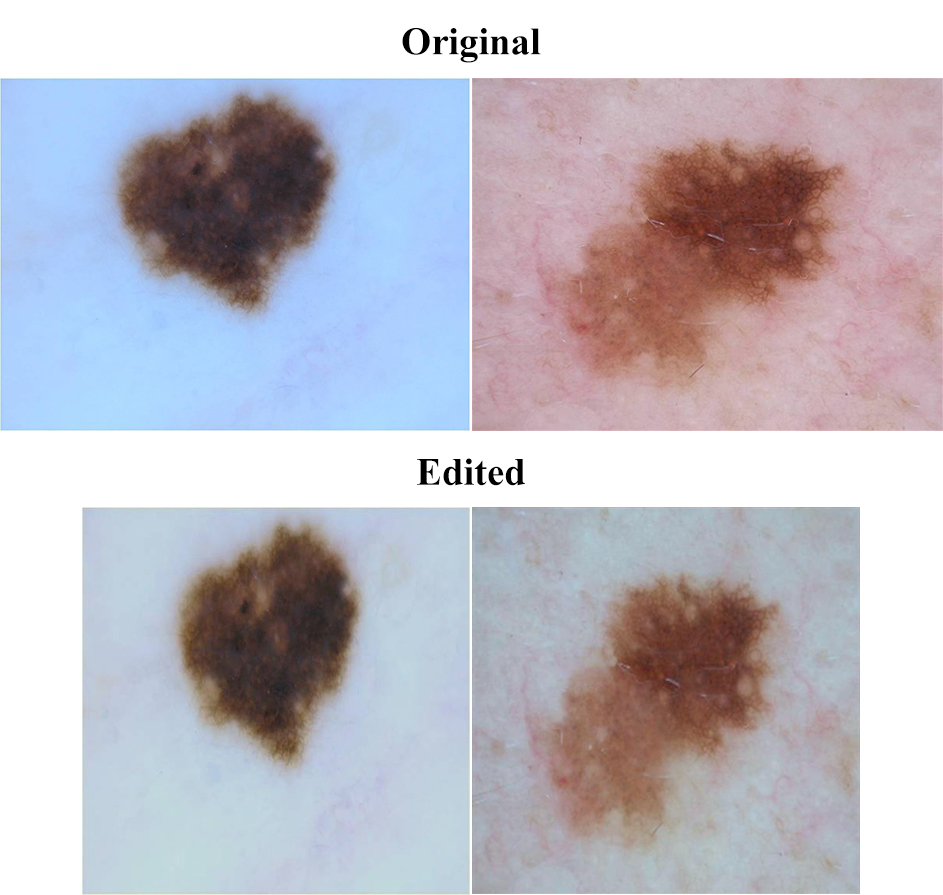
\includegraphics[width=8cm]{SkinLesions.jpg}
\caption{Examples of contrasting pictures, paired with the same pictures after the preprocessing phase.}
\label{fig:skinlesions}
\end{figure}

\begin{figure*}[h]
\centering
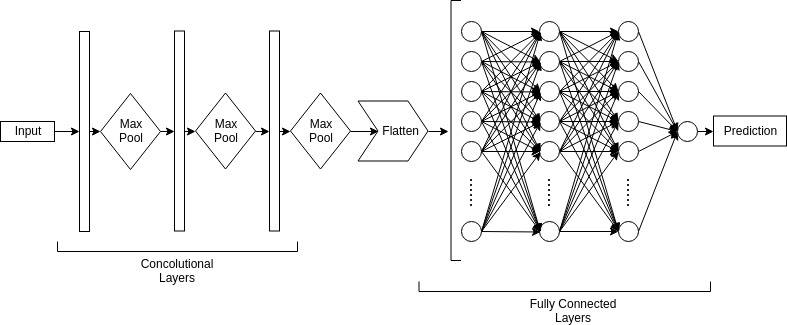
\includegraphics[width=\textwidth, height=7cm]{ModelArchitecture_1Classifier.jpg}
\caption{Architecture of each classifier for the proposed classification model.}
\label{fig:modelarchitecture}
\end{figure*}

\newpage{}
\section{\textbf{Proposed Approach \& Experiments}} %%%%%%%%%%%%%%%%%%%%%%
\label{pae}

Typically, a CNN alternatively stacks convolutional (C) and sub-sampling (e.g. max-pooling) (M) layers. 
In a C layer, small feature extractors (kernels) sweep over the topology and transform the input into feature maps. 
In a M layer, activations within a neighborhood are abstracted to acquire invariance to local translations. 
After several C and M layers, feature maps are flattened into a feature vector, followed by fully-connected (FC) layers. 
The output of these end layers is the final output of the model.

This strategy is the basis of the current state of the art for classification problems using CNNs and image processing.
CNNs have achieved remarkable successes in 2D medical image analysis, as one may ascertain from many studies following this schema.
New approaches tend to explore specific concepts within this standard in order to: proove conjectures, take advantages of those concepts and their characteristics for the case in study, and search for new and improved ways of tackeling machine learning models using CNNs.

\subsection{Proposal for the Classification Model}

The approach that this study offers is a more broad one. 
We aimed to see the effects of several changes to the standard and try to understand the meaning of them.
Figure \ref{fig:modelarchitecture} shows the architecture of each classifier for our final model, for an easier visualization and comprehension.
The two classifiers follow the same architecture.
The network has three convolutional and one pooling layers (with a flattening layer in the end) for feature extraction, and four fully-connected layers (with one dropout in the middle), in the end, for classification. 

The convolutional layers uses the convolution technology itself and it's the core building block of any CNN. 
The main ideia is to iterate over the entire image, not pixel by pixel but using an area approach, i.e. taking in consideration an area of X by X pixels, and produce in the end a N dimensional activation map that represents the evaluation made in every spatial position.

The pooling layer is a common layer to insert in between of succesive convolutional layers.
Sub-sampling (or Pooling) is frequently used in CNNs with the purpose of progressively reducing the spatial size of the representation and thus reducing the amount of features and the computational complexity of the network.
These layers also help in preventing theoverfitting problem and in increasing the speed of convergence.

The flattening layer is very important to make the connection between the convolutional area of the network with the fully connected layers. 
This step is very straightforward, but nevertheless important, consisting basically in transforming the N dimensional tables of features to a vector that the successive layers can operate over.

The fully-connected layers is basically the same as normal DNN, consisting in several neurons in a fully connected layer that have full connections to all activations in the previous layer.

The dropout layer is a layer that applies a technique used to improve over-fit on neural networks, basically during training half or a user defined amount of neurons on a particular layer will be deactivated. This will most of the times improve generalization because forces your layers to learn with different neurons the same "concept".

\subsection{Algorithms Applied}

The whole process from collecting the preprocessed images as input to outputting a class prediction envolves several algorithms with different purposes.

The main purpose of an Activation Function (AF) is to convert a input signal of a node in an ANN to an output signal (used as a input in the next layer).
If no AF is applied, then the output signal is simply a simple linear function - limited in its complexity and less powerful when learning complex functional mappings from big data such as images.
AFs help the model to make sense and extract knowledge form such complicated and non-linear datasets.
\newpage{}
The most common AFs are: 
\begin{itemize}
\item \textbf{Sigmoid or Logistic} - it is a activation function of form \textit{f(x) = 1 / 1 + exp(-x)}. Its range is between 0 and 1. It is a S-shaped curve. It is easy to understand and apply but usually has slow convergence, saturates and kill gradients and makes the gradient updates go too far.
\item \textbf{Hyperbolic Tangent (Tanh)} - its mathematical formula is \textit{f(x) = 1 -  exp(-2x) / 1 + exp(-2x)}. Its output is zero centered because its output ranges between -1 and 1. Hence optimization is easier in this method and, in practice, it is always preferred over Sigmoid function. However, both functions suffer from the Vanishing gradient problem.
\item \textbf{Rectified Linear Units (ReLu)} - it is mathematically represented as \textit{R(x) = max(0,x)}. It has become very popular in the past couple of years since it improves dramatically in convergence speed and avoids and rectifies the vanishing gradient problem. But its limitation is that it should only be used within Hidden layers of an ANN. \textbf{Leaky ReLu} is a modification of this AF to fix the problem of dying neurons (due to fragile gradients during training).
\end{itemize}
Taking this in consideration we decided to apply the Leaky ReLu activation function to all layers except for the final output layer. 

Sub-sampling, already mentioned in the previous subsection, was another algorithm applied in this study.
It is important to be careful in the use of the pooling layer, particularly in vision tasks because, while it would help significantly reduce the complexity of the model, it might cause to lose the location sensitivity in it.
After running a few tests, we came to the conclusion that the lost of location was not a significant problem for our situation and that introducing pooling increased the classifiers' accuracies.
We used the \textbf{MaxPool layer} (the more commonly used pooling layer) of 2x2 - reducing the spatial size to a quarter in each pooling layer.

Flattening has also been discussed in the previous subsection.
In our case, this process was applied to convert the information of the three primary colors (since we are using rgb pictures) into one single vector.
This simplified the data for the remaining network layers.

For accurate predictions, one needs to minimize the ANN's error using back propagation. 
When training, the current error of the ANN is typically propagated backwards to a previous layer, where it is used to modify the weights and bias in such a way that the error is minimized. 
The weights are modified using a function called Optimization Function.
For our model we decided to use \textbf{RMSprop}, a function that lies in the realm of adaptive learning rate methods. 
It basically works as follows: rather than having just a global, scalar learning rate, we have a vector of learning rates for each trainable parameter; it is iteratively updated with a running average of magnitudes of squares of previous gradients. 

\newpage{}
\subsection{Tests \& Results}

Being the first time we ever worked with images and image processing - specially medical images concerning a very important problem as skin cancer is - , we adopted a strategy of trying to learn as much as we possibly could. 
For that we tested various hyperparameters to see what each contributed to the overall performance of our classification model.
The results of the tests were intriguing because some of them didn't correspond with our suppositions. 

It is important to reffer that all tests were made after the preprocessing phase with the step 4 excluded (see chapter \ref{dp}). 
Only the final test took in consideration this final preprocessing step.

An initial version of the classification model was created with an accuracy a bit over 0.75.
For each aspect of the model that we changed, we maintained the remaining unaltered, and all our tests were conducted for the melanoma data only, assuming that the same behavior of the CNN would maintain for the keratosis one.
These two decisions allowed us to save valuable time.

We began the testing phase by studying the influence of the number of epochs, considering numbers  between 30 and 120 varying in steps of 30.
Our observations were that this number was not very relevant given that the accuracy level maintained in between the 0,80 and 0,81 range. 
No lower value was tested as we understood that a minimum number was necessary for the classifier to have "time" to converge to a stable accuracy.

The next number tested was the batch size, which defines the number of divisions of the total data.
Altering between 8, 12 and 16, seemed to have little impact in the results.
An aditional batch size of 2 was tested after that to make sure that, in our case, this component did not have much impact in the training process.
But the accuracy kept in the 0.80 range, with a 0.01 variance.

Another hyperparameter that we considered and that we assumed could be relevant was the kernel size.
This number represents the area that the convolutional layer will process in each step, and turned out to have the some impact in the performance, proven by the fact that when we varied between 3, 4 and 5, the bigger the kernel size was, the lower the accuracy was.
Our observation was backed up by the fact that the bigger the kernel, the less granular the training process will be, and thus important information will be ignored. 

Another component we invested time on trying to optimize was the image.
Given that the images needed to be resized, as mentioned in chapter \ref{dp}, we could test different sizes to see if a bigger image would add information that a smaller sized image could lose in the rescaling process.
But this thought turned out to be false, as after altering between 150x150 pixels and 200x200 pixels, no improvements were visible. 
No larger sizes could be examined due to the memory boundry that we were limited by.

One of the most important aspects to test was the CNN architecture itself, as the reader may easily uderstand.
Like any system composed by several parts (e.g. a car), if the interaction of each part  is somewhat poorly made or their positions are not as they should or there is a lack of important parts, the whole system will not work well.
We quickly noticed that a least good construction of the architecture had catastrofic results.
We experienced this when, were the normal result of models with a minimally good construction rounded the 0.80 accuracy, if we tried to change any aspect of the architecture without a concrete reason the accuracy dropped to 0.50 or lower. 
We tried changing the number of convolutional layers, as well as of fully-connected and activation layers, following the suggestions of one of the articles earlier mentioned, but the performance gains were never very significant, reaching only accuracy values between 0,79 and 0,81.

The last test we ran was one we thought would have a significant improvement, but turned out to do the opposite in our case. 
As explained in chapter \ref{dp}, our fourth preprocessing step was to transform the positive cases of cancer in several ways with the purpose of feeding the model with useful information.
We tried, as many studies in this area suggest, rotating, inverting and transposing the images, increasing the number of data and consequently exposing the model to more options and patterns. 
This ideia seemed to be logical to us in the sense that it would help the model understand more deeply the patterns of the classes of melanoma and keratosis by making the number of occurences of each class closer to each other (as seen in figure \ref{fig:datadistribution2}).
Rotations tested were of 90º, 180º and 270º. Reflections tested were vertical and horizontal.
The result of this test was nothing like wee predicted - on the contrary, the accuracy dropped close to 0,10 from the normal results. 
This result can be linked to something that we do not entirely understand inside the learning process of the CNNs.
Perhaps with a more extensive study of this observation, a solution could be found with results similar to the ones seen in other studies using the same technique.

Finished with all tests, the keratosis classifier was our next target.
Due to the nature of the data, this classifier was doomed to have a weaker performance.
Despite knowing this, we still dedicated some time to tuning this classifier in search of making both DNNs have similar capacities.
\newline{}

No best combination of the most adequate values and configurations was clear, so we had to choose one that we found appropriate amongst the highest performing to build our final model.
As its architecture has already been discussed in the begining of this chapter, we proceed to an analysis of the model's performance.

Regarding the accuracy metric, these are the classifiers results: the validation score for the melanoma classifier was 0.80 and for the keratosis classifier was 0.75; the testing scores were respectively 0.81 and 0.84.
The decrease of the melanoma's accuracy suggests a slight occurence of overfit, however the training accuracy suggests the opposite.
The keratosis classifier seems to have a different behaviour, reaching the highest accuracy score during the final testing.

All code developed during this study was based on the Python library Keras's tools.
We used this library not only to take advantage of its abstraction and ease of use but also to have a stronger assurance of the validity of the results, since Keras is a very famous and well tested library for machine learning using Python.

\newpage{}
\section{\textbf{Conclusions \& Future Work}} %%%%%%%%%%%%%%%%%%%%%%

We present a study that demonstrates the effect of several chances to a classification model and the respective reflections and conclusions taken from them.
Based on the metrics carefully chosen, the final model configuration showed fairly good results, as presented in the previous chapter. 
However, its performance also shows how complex problems such as this are and how dificult it is to achieve market-worthy results. 
This is also visible in researches made on the same topic by more experienced and resourceful investigators, as their models' performances outperform ours only by an average of 10\%.

The tested components with a higher influence on the machine learning model's performance were: the architeture structure, the image transformations and the kernel size.
Although not all behaviours are entirely explained, we believe that putting more time in testing these components and studying deeper the algorithms used in CNNs would bring the accuracy of the model up - with an increase always limited by the nature of the problem.

For future proceedings, some options are promising steps to follow: as concluded during the testing phase, the architecture of a DNN highly affects its error, so a more extensive study on more appropriate architectures could lead to a better model; better data interpretation and perhaps collecting more data from the ISIC archive could help the model learn more patterns and predict with more certainty; exploring gpu capacity to reduce the training time and therefore focus on more important tasks could allow us to test more hyperparameter combinations and bigger sized images.

The repository with the base code developed during this study is available at the University of Aveiro's coding platform (code.ua.pt). 
Link: https://code.ua.pt/git/taa\_proj\_2018-2019
Warning: this link might be updated after this report has been completed.

\begin{thebibliography}{9} %%%%%%%%%%%%%%%%%%%%%%

% Skin Disease Information
\bibitem{nano3}
\emph{Melanoma}, Skin Cancer Foundation
\bibitem{nano3}
\emph{Nevus Treatment}, Healthline
\bibitem{nano3}
\emph{Seborrheic Keratosis Treatment}, Healthline

% Machine Learning Definitions
\bibitem{nano3}
Dr. Saed Sayad, \emph{An Introduction to Data Science}, Rutgers School Computer Science Department: Master Program in Data Science
\bibitem{nano3}
\emph{Artificial Neural Networks}, \emph{Deep Neural Networks}, \emph{Convolutional Neural Networks}, \emph{Perceptron}, \emph{Principal Component Analysis}, definitions taken from Techopedia
\bibitem{nano3}
R. Berwick \& Village Idiot, \emph{Notes on Support Vector Machines}, MIT
\bibitem{nano3}
Niklas Donges, \emph{The Random Forest Algorithm}, Medium: Towards Data Science
\bibitem{nano3}
Prabhu, \emph{Understanding Hyperparameters and its Optimisation Techniques}, Medium: Towards Data Science
\bibitem{nano3}
Aditya Mishra, \emph{Metrics to Evaluate your Machine Learning Algorithm}, Medium: Towards Data Science
\bibitem{nano3}
\emph{Multi-Class Neural Networks: Softmax}, Google Online Course: Multiclass Neural Networks
\bibitem{nano3}
Karpathy, \emph{CS231n Convolutional Neural Networks for Visual Recognition}, Stanford University

% ISIC Challenge
\bibitem{nano3}
The International Skin Imaging Collaboration (ISIC) Website, \emph{ISIC Challenge 2017}, http://challenge2017.isic-archive.com
\bibitem{nano3}
Image Classification of Melanoma, Nevus and Seborrheic Keratosis by Deep Neural Network Ensemble, \emph{ResNet ensemble with normalized image}, Casio and Shinshu University joint team for the ISIC Challenge 2017
\bibitem{nano3}
Incorporating the Knowledge of Dermatologists to Convolutional Neural Networks for the Diagnosis of Skin Lesions, \emph{gpm-LSSSD}, Multimedia Processing Group of the University Carlos III of Madrid

% External Articles
\bibitem{nano3}
A. Namozov and Y. I. Cho, \emph{Improving Dermoscopy Image Classification Using Color Constancy}, International Conference on Information and Communication Technoslogy Convergence (ICTC) 2018
\bibitem{nano3}
A. Namozov and Y. I. Cho, \emph{Convolutional Neural Network Algorithm with Parameterized Activation Function for Melanoma Classification}, International Conference on Information and Communication Technology Convergence (ICTC) 2018 
\bibitem{nano3}
D. Chen, J. Niu, Q. Pan, Y. Li, M. Wang, \emph{A Deep-Learning Based Ultrasound Text Classifier for Predicting Benign and Malignant Thyroid Nodules}, International Conference on Green Informatics (ICGI) 2017
\bibitem{nano3}
Q. Dou, H. Chen, L. Yu, L. Zhao, J. Qin, D. Wang, V. CT Mok, L. Shi, and P. Heng, \emph{Automatic Detection of Cerebral Microbleeds From MR Images via 3D Convolutional Neural Networks}, IEEE Transactions on Medical Imaging 2016, Volume 35, Issue 5
\bibitem{nano3}
N. Srivastava, G. Hinton, A. Krizhevsky, I. Sutskever and R. Salakhutdinov, \emph{Dropout: A Simple Way to Prevent Neural Networks from Overfitting}, University of Toronto Journal of Machine Learning Research 15 (2014)

% Aditional Info
\bibitem{nano3}
The International Skin Imaging Collaboration (ISIC) Website, \emph{ISIC Archive}, https://isic-archive.com.
\bibitem{nano3}
Keras Documentation, https://keras.io/
\bibitem{nano3}
OpenCV Documentation for Python, https://opencv-python-tutroals.readthedocs.io/en/latest/

\end{thebibliography}
\end{document}